\documentclass{article}
\usepackage{amsmath,ifthen,amsthm,amssymb,enumerate}
\usepackage[margin=1in]{geometry}
\usepackage[colorlinks=true,linkcolor=blue]{hyperref}
\usepackage{tikz,pgfplots}
\usepackage{tbil-de}
%\usetikzlibrary{external}
%\tikzexternalize 
%\tikzsetexternalprefix{aux/}

\newenvironment{problem}[1]
{
	\textbf{#1.}
	\ignorespaces
}{
\vspace{0.2in}
}

\newenvironment{solution}
{
	\textit{Solution.}
	\ignorespaces
}{
	\qed

	\vspace{1em}
}

\newcommand{\startModule}[1]
{
	\section*{Module #1}
	\addcontentsline{toc}{section}{Module #1}
}
\newcommand{\startStandard}[1]
{
	\subsection*{Standard #1}
	\addcontentsline{toc}{subsection}{Standard #1}
}

\begin{document}
\begin{flushleft}

\startModule{C}
\startStandard{C1}
\begin{problem}{C1}
Sketch a solution curve through each point marked in the slope field.

\begin{center}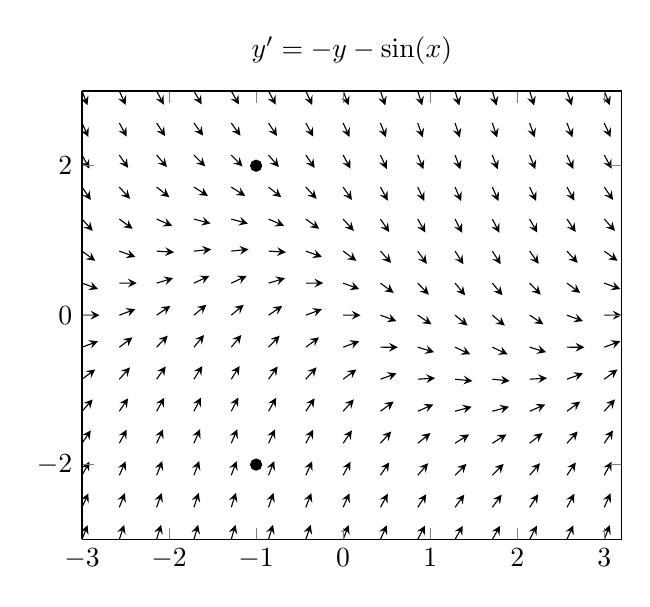
\begin{tikzpicture}
    \begin{axis}[
        title={\(y' = -y - \sin(x)\)},
        domain=-3:3,
        view={0}{90},
        axis background/.style={fill=white},
    ]
        \addplot3[black,
            quiver={
             u={1/(sqrt(1 + (-y - sin(60*x))^2)},
             v={(-y - sin(60*x))/(sqrt(1 + (-y - sin(60*x))^2)},
             scale arrows=0.2,
            },
            -stealth,samples=15]
                {exp(-x) - 1/2*sin(x) - 1/2*cos(x)};
        %KAWWWWWWW
        % Here be some points added to the swoopy loop vector fieldamagigs
        \addplot[mark=*] coordinates {(-1,2)}; % Obvious ordered pair for lococation
        \addplot[mark=*] coordinates {(-1,-2)};
    \end{axis}
\end{tikzpicture}\end{center}
\end{problem}

\begin{problem}{C1}
Sketch a solution curve through each point marked in the slope field.

\begin{center}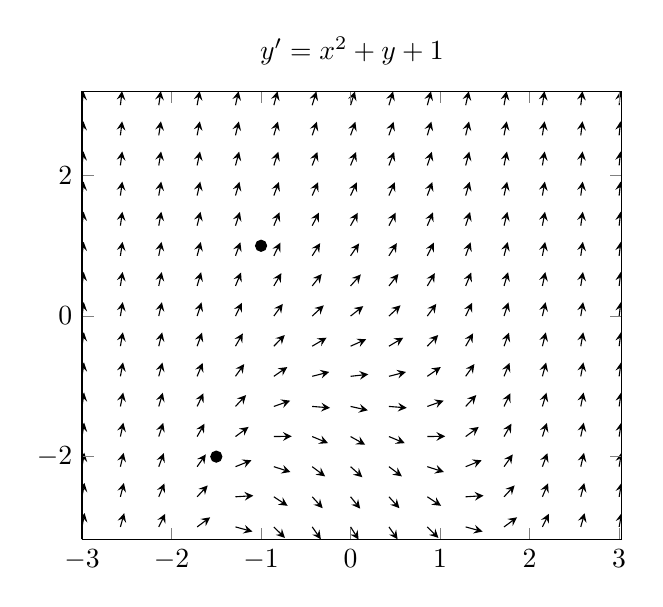
\begin{tikzpicture}
    \begin{axis}[
        title={\(y' = x^2 + y+1\)},
        domain=-3:3,
        view={0}{90},
        axis background/.style={fill=white},
    ]
        \addplot3[black,
            quiver={
             u={1/sqrt(1 + (x^2+y+1)^2)},
             v={(x^2 + y+1)/sqrt(1 + (x^2+y+1)^2)},
             scale arrows=0.2,
            },
            -stealth,samples=15]
                {exp(x) - x - 1};
        %KAWWWWWWW
        % Here be some points added to the swoopy loop vector fieldamagigs
        \addplot[mark=*] coordinates {(-1,1)}; % Obvious ordered pair for lococation
        \addplot[mark=*] coordinates {(-1.5,-2)};
    \end{axis}
\end{tikzpicture}\end{center}
\end{problem}

\begin{problem}{C1}
Sketch a solution curve through each point marked in the slope field.

\begin{center}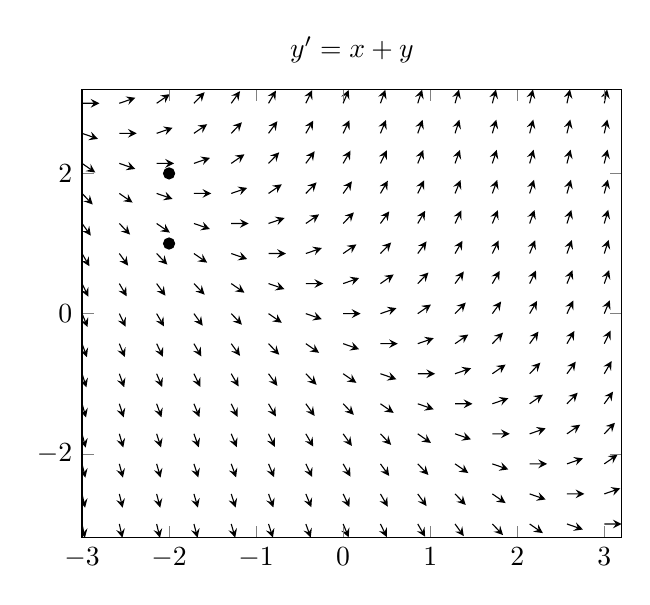
\begin{tikzpicture}
    \begin{axis}[
        title={\(y' = x + y\)},
        domain=-3:3,
        view={0}{90},
        axis background/.style={fill=white},
    ]
        \addplot3[black,
            quiver={
             u={1/sqrt(1 + (x+y)^2)},
             v={(x + y)/sqrt(1 + (x+y)^2)},
             scale arrows=0.2,
            },
            -stealth,samples=15]
                {exp(x) - x - 1};
        %KAWWWWWWW
        % Here be some points added to the swoopy loop vector fieldamagigs
        \addplot[mark=*] coordinates {(-2,1)}; % Obvious ordered pair for lococation
        \addplot[mark=*] coordinates {(-2,2)};
    \end{axis}
\end{tikzpicture}\end{center}
\end{problem}

\begin{problem}{C1}
Sketch a solution curve through each point marked in the slope field.

\begin{center}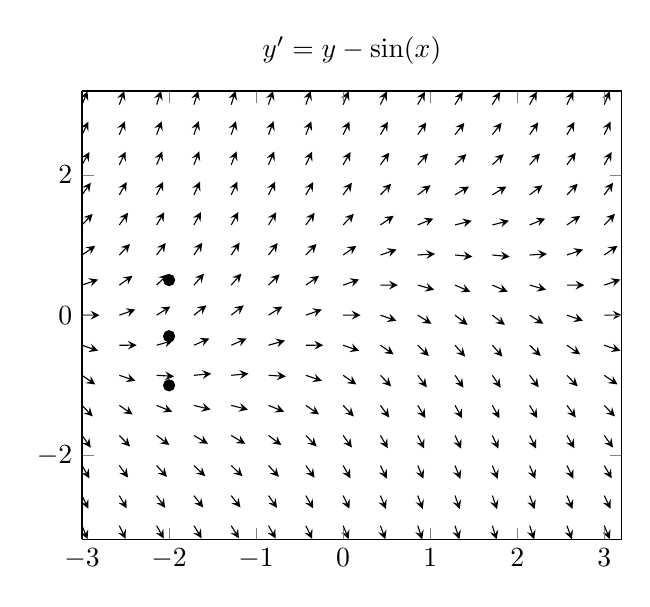
\begin{tikzpicture}
    \begin{axis}[
        title={\(y' = y - \sin(x)\)},
        domain=-3:3,
        view={0}{90},
        axis background/.style={fill=white},
    ]
        \addplot3[black,
            quiver={
             u={1/sqrt(1 + (y-sin(60*x))^2)},
             v={(y - sin(60*x))/sqrt(1 + (y-sin(60*x))^2)},
             scale arrows=0.2,
            },
            -stealth,samples=15]
                {exp(x) + 1/2*sin(x) + 1/2*cos(x)};
        %KAWWWWWWW
        % Here be some points added to the swoopy loop vector fieldamagigs
        \addplot[mark=*] coordinates {(-2,-1)}; % Obvious ordered pair for lococation
        \addplot[mark=*] coordinates {(-2,-.3)};
        \addplot[mark=*] coordinates {(-2,.5)};
    \end{axis}
\end{tikzpicture}\end{center}
\end{problem}

\begin{problem}{C1}
Sketch a solution curve through each point marked in the slope field.

\begin{center}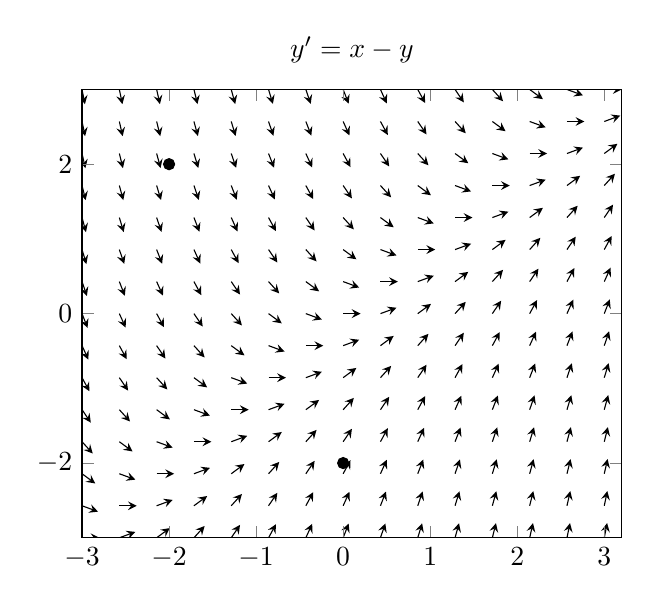
\begin{tikzpicture}
    \begin{axis}[
        title={\(y' = x - y\)},
        domain=-3:3,
        view={0}{90},
        axis background/.style={fill=white},
    ]
        \addplot3[black,
            quiver={
             u={1/sqrt(1 + (x - y)^2)},
             v={(x - y)/sqrt(1 + (x - y)^2)},
             scale arrows=0.2,
            },
            -stealth,samples=15]
                {exp(-x) + x - 1};
        \addplot[mark=*] coordinates {(-2,2)};
        \addplot[mark=*] coordinates {(0,-2)};
    \end{axis}
\end{tikzpicture}\end{center}
\end{problem}

\begin{problem}{C1}
Sketch a solution curve through each point marked in the slope field.

\begin{center}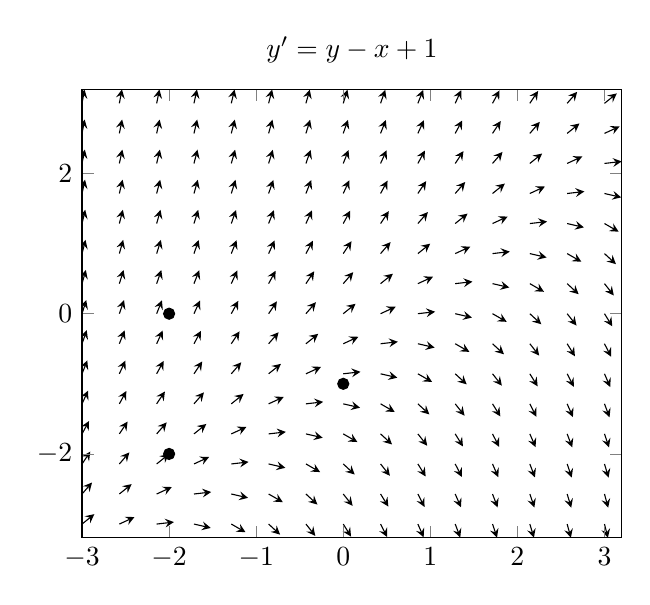
\begin{tikzpicture}
    \begin{axis}[
        title={\(y' = y - x + 1\)},
        domain=-3:3,
        view={0}{90},
        axis background/.style={fill=white},
    ]
        \addplot3[black,
            quiver={
             u={1/sqrt(1 + (y - x + 1)^2)},
             v={(y - x + 1)/sqrt(1 + (y - x + 1)^2)},
             scale arrows=0.2,
            },
            -stealth,samples=15]
                {exp(x) + x};
        \addplot[mark=*] coordinates {(-2,-2)};
        \addplot[mark=*] coordinates {(-2,0)};
        \addplot[mark=*] coordinates {(0,-1)};
    \end{axis}
\end{tikzpicture}\end{center}
\end{problem}

\begin{problem}{C1}
Sketch a solution curve through each point marked in the slope field.

\begin{center}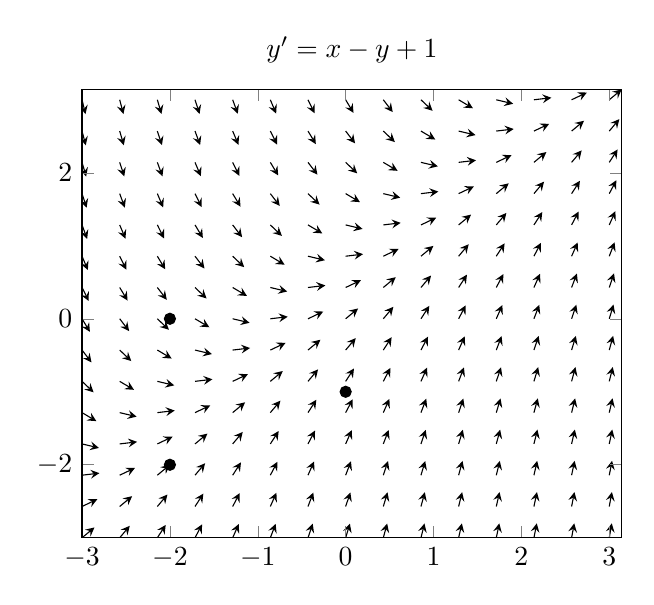
\begin{tikzpicture}
    \begin{axis}[
        title={\(y' = x - y + 1\)},
        domain=-3:3,
        view={0}{90},
        axis background/.style={fill=white},
    ]
        \addplot3[black,
            quiver={
             u={1/sqrt(1 + (x - y + 1)^2)},
             v={(x - y + 1)/sqrt(1 + (x - y + 1)^2)},
             scale arrows=0.2,
            },
            -stealth,samples=15]
                {exp(-x) + x};
        \addplot[mark=*] coordinates {(-2,-2)};
        \addplot[mark=*] coordinates {(-2,0)};
        \addplot[mark=*] coordinates {(0,-1)};
    \end{axis}
\end{tikzpicture}\end{center}
\end{problem}

\begin{problem}{C1}
Sketch a solution curve through each point marked in the slope field.

\begin{center}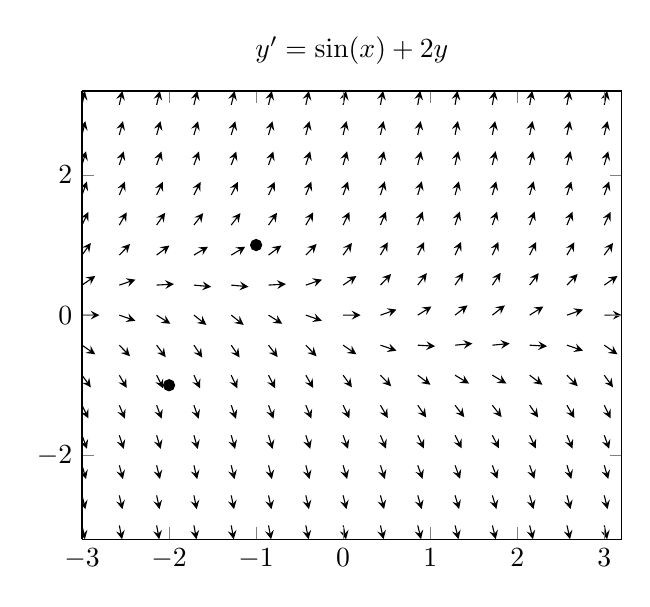
\begin{tikzpicture}
    \begin{axis}[
        title={\(y' = \sin(x) + 2y\)},
        domain=-3:3,
        view={0}{90},
        axis background/.style={fill=white},
    ]
        \addplot3[black,
            quiver={
             u={1/sqrt(1 + (sin(60*x) + 2*y)^2)},
             v={(sin(60*x) +2*y)/sqrt(1 + (sin(60*x) + 2*y)^2)},
             scale arrows=0.2,
            },
            -stealth,samples=15]
                {x};
        \addplot[mark=*] coordinates {(-1,1)};
        \addplot[mark=*] coordinates {(-2,-1)};
    \end{axis}
\end{tikzpicture}\end{center}
\end{problem}

\begin{problem}{C1}
Sketch a solution curve through each point marked in the slope field.

\begin{center}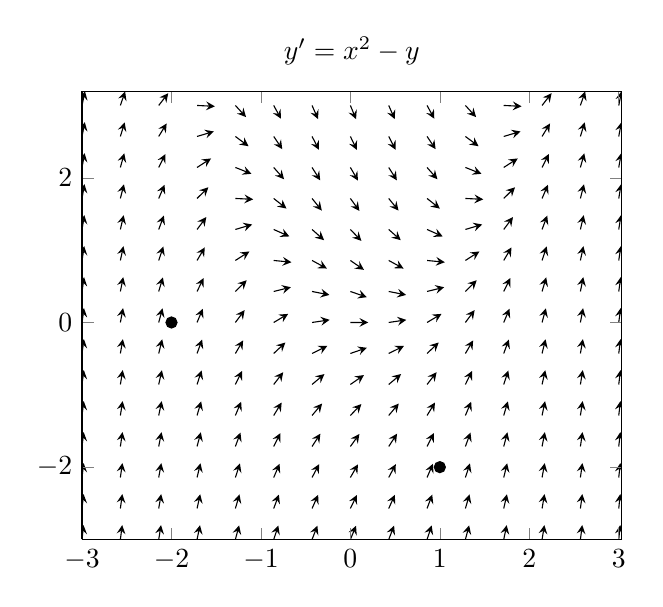
\begin{tikzpicture}
    \begin{axis}[
        title={\(y' = x^2 - y\)},
        domain=-3:3,
        view={0}{90},
        axis background/.style={fill=white},
    ]
        \addplot3[black,
            quiver={
             u={1/sqrt(1 + (x^2 - y)^2)},
             v={(x^2 - y)/sqrt(1 + (x^2 - y)^2)},
             scale arrows=0.2,
            },
            -stealth,samples=15]
                {x};
        \addplot[mark=*] coordinates {(-2,0)};
        \addplot[mark=*] coordinates {(1,-2)};
    \end{axis}
\end{tikzpicture}\end{center}
\end{problem}

 \newpage
\begin{problem}{C2}
Set up and solve a differential equation to answer the following question: \\
A water droplet with a radius of \(100\ {\rm \mu m}\) has a mass of about \(4 \times 10^{-12} {\rm kg}\) and a terminal velocity of \(27\ {\rm \frac{cm}{s}}\).  Such a droplet is dropped from rest.  What is its velocity after \(0.01\ {\rm s}\)?
\end{problem}

\begin{problem}{C2}
Set up and solve a differential equation to answer the following question: \\
A water droplet with a radius of \(100\ {\rm \mu m}\) has a mass of about \(4 \times 10^{-12} {\rm kg}\).  Such a droplet is dropped from rest.  After \(0.02\ {\rm s}\) it has reached half of its terminal velocity.  What is its terminal velocity?
\end{problem}

\begin{problem}{C2}
Set up and solve a differential equation to answer the following question: \\
A water droplet with a radius of \(10\ {\rm \mu m}\) has a mass of about \(4 \times 10^{-15} {\rm kg}\).  Such a droplet is dropped from rest.  After \(0.002\ {\rm s}\) it has reached half of its terminal velocity.  What is its terminal velocity?
\end{problem}

\begin{problem}{C2}
Set up and solve a differential equation to answer the following question: \\
A single grain of corn pollen has a radius of \(50\ {\rm \mu m}\) and a terminal velocity of \(27\ {\rm \frac{cm}{s}}\).  Such a droplet is dropped from rest.  What is its velocity after \(0.01\ {\rm s}\)?
\end{problem}
 \newpage
\begin{problem}{C3}
Find the general solution to
\[
y'' + 2y' + y = 0.
\]
\end{problem}

\begin{problem}{C3}
Find the general solution to
\[
y'' + 2y' - 8y = 0.
\]
\end{problem}

\begin{problem}{C3}
Find the general solution to
\[
y'' + 4y' + 3y = 0.
\]
\end{problem}

\begin{problem}{C3}
Find the general solution to
\[
y'' + 2y' - 3y = 0.
\]
\end{problem}

\begin{problem}{C3}
Find the general solution to
\[
y'' - 2y' - 3y = 0.
\]
\end{problem}

\begin{problem}{C3}
Find the general solution to
\[
y'' + 4y' + 4y = 0.
\]

\end{problem}

\begin{problem}{C3}
Find the general solution to
\[
y'' - 4y' + 4y = 0.
\]
\end{problem}

\begin{problem}{C3}
Find the general solution to
\[
y'' + 5y' + 6y = 0.
\]
\end{problem}


%Add more complex roots
\begin{problem}{C3}
Find the general solution to
\[
y'' - 2y' + 2y = 0.
\]
\end{problem}

\begin{problem}{C3}
Find the general solution to
\[
y'' + 2y' + 2y = 0.
\]
\end{problem}
 \newpage
\begin{problem}{C4}
Find the general solution to
\[
y'' + 2y' + y = 0.
\]
\end{problem}

\begin{problem}{C4}
Find the general solution to
\[
y'' + 2y' - 8y = 0.
\]
\end{problem}

\begin{problem}{C4}
Find the general solution to
\[
y'' + 4y' + 3y = 0.
\]
\end{problem}

\begin{problem}{C4}
Find the general solution to
\[
y'' + 2y' - 3y = 0.
\]
\end{problem}

\begin{problem}{C4}
Find the general solution to
\[
y'' - 2y' - 3y = 0.
\]
\end{problem}

\begin{problem}{C4}
Find the general solution to
\[
y'' + 4y' + 4y = 0.
\]

\end{problem}

\begin{problem}{C4}
Find the general solution to
\[
y'' - 4y' + 4y = 0.
\]
\end{problem}

\begin{problem}{C4}
Find the general solution to
\[
y'' + 5y' + 6y = 0.
\]
\end{problem}


%Add more complex roots
\begin{problem}{C4}
Find the general solution to
\[
y'' - 2y' + 2y = 0.
\]
\end{problem}

\begin{problem}{C4}
Find the general solution to
\[
y'' + 2y' + 2y = 0.
\]
\end{problem}

\begin{problem}{C4}
Find the general solution to
\[
y'' - 6y' + 10y = 0.
\]
\end{problem}

\begin{problem}{C4}
Find the general solution to
\[
y'' + 6y' + 10y = 0.
\]
\end{problem}

\begin{problem}{C4}
Find the general solution to
\[
y'' - 2y' + 5y = 0.
\]
\end{problem}

\begin{problem}{C4}
Find the general solution to
\[
y'' + 2y' + 5y = 0.
\]
\end{problem}

\begin{problem}{C4}
Find the general solution to
\[
y'' - 4y' + 5y = 0.
\]
\end{problem}

\begin{problem}{C4}
Find the general solution to
\[
y'' + 4y' + 5y = 0.
\]
\end{problem}
 \newpage
\begin{problem}{C5}
Find the solution to
\[
y'' + 2y' + y = 0 
\]
when \(y(0)=0\) and \(y'(0)=2\).
\end{problem}

\begin{problem}{C5}
Find the solution to
\[
y'' + 2y' + y = 0 
\]
when \(y(0)=2\) and \(y'(0)=0\).
\end{problem}

\begin{problem}{C5}
Find the solution to
\[
y'' + 2y' - 8y = 0
\]
when \(y(0)=3\) and \(y'(0)=-6\).
\end{problem}

\begin{problem}{C5}
Find the solution to
\[
y'' + 4y' + 3y = 0
\]
when \(y(0)=1\) and \(y'(0)=5\).
\end{problem}

\begin{problem}{C5}
Find the solution to
\[
y'' + 2y' - 3y = 0
\]
when \(y(0)=5\) and \(y'(0)=1\).
\end{problem}

\begin{problem}{C5}
Find the solution to
\[
y'' + 2y' - 3y = 0
\]
when \(y(0)=2\) and \(y'(0)=2\).
\end{problem}

\begin{problem}{C5}
Find the solution to
\[
y'' - 2y' - 3y = 0
\]
when \(y(0)=2\) and \(y'(0)=2\).
\end{problem}

\begin{problem}{C5}
Find the solution to
\[
y'' + 4y' + 4y = 0
\]
when \(y(0)=1\) and \(y'(0)=3\).
\end{problem}

\begin{problem}{C5}
Find the solution to
\[
y'' - 4y' + 4y = 0
\]
when \(y(0)=1\) and \(y'(0)=3\).
\end{problem}

\begin{problem}{C5}
Find the solution to
\[
y'' + 4y' + 4y = 0
\]
when \(y(0)=3\) and \(y'(0)=1\).
\end{problem}

\begin{problem}{C5}
Find the solution to
\[
y'' - 4y' + 4y = 0
\]
when \(y(0)=3\) and \(y'(0)=1\).
\end{problem}

\begin{problem}{C5}
Find the solution to
\[
y'' + 5y' + 6y = 0
\]
when \(y(0)=3\) and \(y'(0)=1\).
\end{problem}

\begin{problem}{C5}
Find the solution to
\[
y'' + 5y' + 6y = 0
\]
when \(y(0)=1\) and \(y'(0)=2\).
\end{problem}

 \newpage
%\begin{problem}{C6}
Find the solution to
\[
y'' + 2y' + y = 0 
\]
when \(y(0)=0\) and \(y'(0)=2\).
\end{problem}

\begin{problem}{C6}
Find the solution to
\[
y'' + 2y' + y = 0 
\]
when \(y(0)=2\) and \(y'(0)=0\).
\end{problem}

\begin{problem}{C6}
Find the solution to
\[
y'' + 2y' - 8y = 0
\]
when \(y(0)=3\) and \(y'(0)=-6\).
\end{problem}

\begin{problem}{C6}
Find the solution to
\[
y'' + 4y' + 3y = 0
\]
when \(y(0)=1\) and \(y'(0)=5\).
\end{problem}

\begin{problem}{C6}
Find the solution to
\[
y'' + 2y' - 3y = 0
\]
when \(y(0)=5\) and \(y'(0)=1\).
\end{problem}

\begin{problem}{C6}
Find the solution to
\[
y'' + 2y' - 3y = 0
\]
when \(y(0)=2\) and \(y'(0)=2\).
\end{problem}

\begin{problem}{C6}
Find the solution to
\[
y'' - 2y' - 3y = 0
\]
when \(y(0)=2\) and \(y'(0)=2\).
\end{problem}

\begin{problem}{C6}
Find the solution to
\[
y'' + 4y' + 4y = 0
\]
when \(y(0)=1\) and \(y'(0)=3\).
\end{problem}

\begin{problem}{C6}
Find the solution to
\[
y'' - 4y' + 4y = 0
\]
when \(y(0)=1\) and \(y'(0)=3\).
\end{problem}

\begin{problem}{C6}
Find the solution to
\[
y'' + 4y' + 4y = 0
\]
when \(y(0)=3\) and \(y'(0)=1\).
\end{problem}

\begin{problem}{C6}
Find the solution to
\[
y'' - 4y' + 4y = 0
\]
when \(y(0)=3\) and \(y'(0)=1\).
\end{problem}

\begin{problem}{C6}
Find the solution to
\[
y'' + 5y' + 6y = 0
\]
when \(y(0)=3\) and \(y'(0)=1\).
\end{problem}

\begin{problem}{C6}
Find the solution to
\[
y'' + 5y' + 6y = 0
\]
when \(y(0)=1\) and \(y'(0)=2\).
\end{problem}

 \newpage

\startModule{F}
\startStandard{F1}
\begin{problem}{V1}
Let \(V\) be the  set of all real numbers together with the operations \(\oplus\) and \(\odot\) defined by, for any \(x,y\in V\) and \(c\in \IR\),
\begin{align*}
x\oplus y  &= x+y \\
c \odot x &= cx-3(c-1)
\end{align*}
\begin{enumerate}[(a)]
\item Show that \textbf{scalar multiplication} is
      \textbf{associative}: \(a\odot(b\odot x)=(ab)\odot x\) for all scalars \(a,b \in \IR\) and \(x \in V\).
\item Show that scalar multiplication does not distribute over vector addition, i.e. for some scalar \(a \in \IR\) and \(x,y\in V\), \(a \odot (x \oplus y) \neq a \odot x \oplus a \odot y\).
\end{enumerate}
\end{problem}


\begin{problem}{V1}
Let \(V\) be the set of all pairs of real numbers with the operations, for any \((x_1,x_2), (y_1,y_2) \in V\), \(c\in \IR\),
\begin{align*}
(x_1,x_2) \oplus (y_1,y_2) &= (x_1+y_1,x_2+y_2+2x_1y_1) \\
c \odot (x_1,x_2) &= (cx_1, cx_2)
\end{align*}
\begin{enumerate}[(a)]
\item Show that the vector \textbf{addition} \(\oplus\) is \textbf{associative}:
      \((x_1,x_2) \oplus ((y_1,y_2) \oplus (z_1,z_2))=((x_1,x_2)\oplus (y_1,y_2))\oplus (z_1,z_2)\) for all \((x_1,x_2), (y_1,y_2), (z_1,z_2) \in V\).
\item Show that scalar multiplication does not distribute over scalar addition, i.e. for some scalars \(a,b \in \IR\) and \((x_1,x_2) \in V\), \( (a+b) \odot (x_1,x_2) \neq a\odot (x_1,x_2) \oplus b \odot (x_1,x_2) \).
\end{enumerate}
\end{problem}



\begin{problem}{V1}
Let \(V\) be the set of all pairs of real numbers with the operations, for any \((x_1,x_2), (y_1,y_2) \in V\), \(c\in \IR\),
\begin{align*}
(x_1,x_2) \oplus (y_1,y_2) &= (x_1+y_1-1,x_2+y_2-1) \\
c \odot (x_1,x_2) &= (cx_1, cx_2)
\end{align*}
\begin{enumerate}[(a)]
\item Show that this vector space has an \textbf{additive identity} element, i.e. an element
      \(\mathbf{z} \in V\) satisfying \((x,y)\oplus\mathbf{z}=(x,y)\) for every \((x,y) \in V\).
\item Show that scalar multiplication does not distribute over vector addition, i.e. for some \(a \in \IR\) and \( (x_1,x_2), (y_1,y_2) \in V\), \(a \odot \left( (x_1,x_2)\oplus (y_1,y_2) \right) \neq a \odot (x_1,x_2) \oplus a \odot (y_1,y_2) \).
\end{enumerate}
\end{problem}

\begin{problem}{V1}
Let \(V\) be the set of all pairs of real numbers with the operations, for any \((x_1,x_2), (y_1,y_2) \in V\), \(c\in \IR\),
\begin{align*}
(x_1,x_2) \oplus (y_1,y_2) &= (x_1+y_1,x_2+y_2) \\
c \odot (x_1,x_2) &= (0, cx_2)
\end{align*}
\begin{enumerate}[(a)]
\item Show that \textbf{scalar multiplication
      distributes over scalar addition}, i.e. that
      \((c+d)\odot(x_1,x_2)=
      c\odot(x_1,x_2) \oplus d\odot(x_1,x_2)\) for every \(c,d \in \IR\) and \( (x_1,x_2) \in V\).
\item Show that 1 is not a scalar multiplicative identity.
\end{enumerate}
\end{problem}


 \begin{problem}{V1}
 Let \(V\) be the set of all pairs of real numbers with the operations, for any \((x_1,x_2), (y_1,y_2) \in V\), \(c\in \IR\),
 \begin{align*}
 (x_1,x_2) \oplus (y_1,y_2) &= (x_1+y_1,x_2+y_2) \\
 c \odot (x_1,x_2) &= (c^2x_1, c^3x_2)
 \end{align*}
 \begin{enumerate}[(a)]
 \item Show that \textbf{scalar multiplication distributes over
       vector addition}, i.e. that
       \(c\odot((x_1,x_2) \oplus (y_1,y_2))=
       c\odot(x_1,x_2) \oplus c\odot(y_1,y_2)\) for all \(c \in \IR\) and \( (x_1,x_2), (y_1,y_2) \in V\).
 \item Show that scalar multiplication does not distribute over
       scalar addition, i.e. for some \(c,d \in \IR\) and \( (x_1,x_2)\in V\)
       \((c+d)\odot(x_1,x_2)\neq c\odot(x_1,x_2) \oplus d\odot(x_1,x_2)\).
 \end{enumerate}
\end{problem}
%
%
% \begin{problem}{V1}
% Let \(V\) be the set of all polynomials with the operations, for any \(f,g\in V\), \(c\in \IR\),
% \begin{align*}
% f \oplus g &= f^\prime + g^\prime \\
% c \odot f &= c f^\prime
% \end{align*}
% (here \(f^\prime\) denotes the derivative of \(f\)).
% \begin{enumerate}[(a)]
% \item Show that scalar multiplication distributes over
%       vector addition, i.e. for all \(c\in \IR\) and \(f,g \in V\)
%       \(c\odot(f \oplus g)=
%       c\odot f \oplus c\odot g\).
% \item  Show that there is no additive identity element.
% \end{enumerate}
% \end{problem}
% \begin{solution}
% Let \(f,g \in \mathcal{P}\), and let \(c\in \IR\).
% \[c \odot (f \oplus g) = c \odot (f^\prime+g^\prime) =
% c(f^\prime+g^\prime)^\prime = cf^{\prime\ \prime}+cg^{\prime\ \prime} =
% cf^\prime\oplus cg^\prime= c \odot f \oplus c \odot g.\]
% However, this is not a vector space, as there is no zero vector.  Additionally, \(1 \odot f \neq f\) for any nonzero polynomial \(f\).
% \end{solution}
%
%
 \begin{problem}{V1}
 Let \(V\) be the set of all real numbers with the operations, for any \(x,y\in V\), \(c\in \IR\),
 \begin{align*}
 x \oplus y &= \sqrt{x^2+y^2} \\
 c \odot x &= c x
 \end{align*}
 \begin{enumerate}[(a)]
 \item Show that the \textbf{vector addition \(\oplus\) is associative}, i.e. that \(x \oplus (y \oplus z)=(x\oplus y)\oplus z\) for all \(x,y,z \in V\).

 \item  Show that there is no additive identity element, i.e. there is no element \(\mathbf{z} \in V\) such that \(x \oplus \mathbf{z} = x\) for all \(x \in V\).
 \end{enumerate}
 \end{problem}

 \begin{problem}{V1}
 Let \(V\) be the set of all pairs of real numbers with the operations, for any \((x_1,x_2), (y_1,y_2) \in V\), \(c\in \IR\),
 \begin{align*}
 (x_1,x_2) \oplus (y_1,y_2) &= (x_1+y_1,x_2y_2) \\
 c \odot (x_1,x_2) &= (cx_1, cx_2)
 \end{align*}
 \begin{enumerate}[(a)]
 \item Show that there is an \textbf{additive identity element}, i.e. an element \(\mathbf{z} \in V\) such that \((x_1,x_2)\oplus\vec{z}= (x_1,x_2)\) for any \( (x_1,x_2) \in V\).
\item Show that scalar multiplication does not distribute over vector addition, i.e. for some \(a \in \IR\) and \( (x_1,x_2), (y_1,y_2) \in V\), that \(a \odot \left( (x_1,x_2)\oplus (y_1,y_2) \right) \neq a \odot (x_1,x_2) \oplus a \odot (y_1,y_2) \).
 \end{enumerate}
\end{problem}
 \newpage
\begin{problem}{F2}
Find the general solution to \(\frac{dy}{dx} + 3xy = 0\).
\end{problem}

\begin{problem}{F2}
Find the general solution to \(y' - y\sin(x)=0\).
\end{problem} 

\begin{problem}{F2}
Find the general solution to \(y' - y^2e^x=0\).
\end{problem} 

\begin{problem}{F2}
Find the general solution to \(y' = \frac{x+2}{y^2}\).
\end{problem}


\begin{problem}{F2}
Find the general solution to \(xy' = y\).
\end{problem}

\begin{problem}{F2}
Find the general solution to \(y\frac{dy}{dx} = y^2\cos(x)\).
\end{problem}

\begin{problem}{F2}
Find the general solution to \(xy^2\frac{dy}{dx} = 1\).
\end{problem}

\begin{problem}{F2}
Find the general solution to \(x\cos(y)y' = 1\).
\end{problem}
 \newpage
%\begin{problem}{F3}
Find the general solution to \(xy' + 4y = 2x\).
\end{problem}

\begin{problem}{F3}
Find the general solution to \(xy' + 4y = \sqrt{x}\) (for $x>0$).
\end{problem}

\begin{problem}{F3}
Find the general solution to \(xy' + 2y = x^2\).
\end{problem}

\begin{problem}{F3}
Find the general solution to \(y' = 2 + x + 2y + xy\).
\end{problem}

\begin{problem}{F3}
Find the general solution to \(y' = 1 + 2x + y + 2xy\).
\end{problem}

 \newpage


\begin{problem}{F4}
One of the two ODEs below is exact.  Identify which one, and solve it.
\begin{align*}
 (x + 2y)y'+y &=2x \\ %Exact
 (x + 2y)y'-y &=-2x  
\end{align*}
\end{problem}

\begin{problem}{F4}
One of the two ODEs below is exact.  Identify which one, and solve it.
\begin{align*}
(3x + 2y)y'+3y &= 2x \\ %Exact
(3x + 2y)y'-3y &= -2x  
\end{align*}
\end{problem}

\begin{problem}{F4}
One of the two ODEs below is exact.  Identify which one, and solve it.
\begin{align*}
(x^2 + 3y^2)y' -2xy &= -3x^2 \\
(x^2 + 3y^2)y' +2xy &= 3x^2  %Exact
\end{align*}
\end{problem}

\begin{problem}{F4}
One of the two ODEs below is exact.  Identify which one, and solve it.
\begin{align*}
(2xy + 3y^2)y' +y^2 &= 3x^2\\ %Exact
(2xy + 3y^2)y' -y^2 &= -3x^2
\end{align*}
\end{problem}

\begin{problem}{F4}
One of the two ODEs below is exact.  Identify which one, and solve it.
\begin{align*}
\cos(x)\cos(y)y' &= \sin(x)\sin(y) \\ %Exact
\cos(x)\cos(y)y' &= \sin(x)+\sin(y)
\end{align*}
\end{problem}

\begin{problem}{F4}
One of the two ODEs below is exact.  Identify which one, and solve it.
\begin{align*}
\sin(x)\sin(y)y' = \cos(x)+\cos(y) \\
\sin(x)\sin(y)y' = \cos(x)\cos(y)  %Exact
\end{align*}
\end{problem}

\begin{problem}{F4}
One of the two ODEs below is exact.  Identify which one, and solve it.
\begin{align*}
(y^3e^x+xe^x)y' +3e^xy^2 = 3x^2\\
(2ye^x+e^y)y' +e^xy^2 = 3x^2 %Exact
\end{align*}
\end{problem}


 \newpage
\begin{problem}{F5}
Find the general solution to \(xy' + 4y = 2x\).
\end{problem}

\begin{problem}{F5}
Find the general solution to \(xy' + 4y = \sqrt{x}\) (for \(x>0\)).
\end{problem}

\begin{problem}{F5}
Find the general solution to \(xy' + 2y = x^2\).
\end{problem}


 \newpage


\begin{problem}{F6}
One of the two ODEs below is exact.  Identify which one, and solve it.
\begin{align*}
 (x + 2y)y'+y &=2x \\ %Exact
 (x + 2y)y'-y &=-2x  
\end{align*}
\end{problem}

\begin{problem}{F6}
One of the two ODEs below is exact.  Identify which one, and solve it.
\begin{align*}
(3x + 2y)y'+3y &= 2x \\ %Exact
(3x + 2y)y'-3y &= -2x  
\end{align*}
\end{problem}

\begin{problem}{F6}
One of the two ODEs below is exact.  Identify which one, and solve it.
\begin{align*}
(x^2 + 3y^2)y' -2xy &= -3x^2 \\
(x^2 + 3y^2)y' +2xy &= 3x^2  %Exact
\end{align*}
\end{problem}

\begin{problem}{F6}
One of the two ODEs below is exact.  Identify which one, and solve it.
\begin{align*}
(2xy + 3y^2)y' +y^2 &= 3x^2\\ %Exact
(2xy + 3y^2)y' -y^2 &= -3x^2
\end{align*}
\end{problem}

\begin{problem}{F6}
One of the two ODEs below is exact.  Identify which one, and solve it.
\begin{align*}
\cos(x)\cos(y)y' &= \sin(x)\sin(y) \\ %Exact
\cos(x)\cos(y)y' &= \sin(x)+\sin(y)
\end{align*}
\end{problem}

\begin{problem}{F6}
One of the two ODEs below is exact.  Identify which one, and solve it.
\begin{align*}
\sin(x)\sin(y)y' = \cos(x)+\cos(y) \\
\sin(x)\sin(y)y' = \cos(x)\cos(y)  %Exact
\end{align*}
\end{problem}

\begin{problem}{F6}
One of the two ODEs below is exact.  Identify which one, and solve it.
\begin{align*}
(y^3e^x+xe^x)y' +3e^xy^2 = 3x^2\\
(2ye^x+e^y)y' +e^xy^2 = 3x^2 %Exact
\end{align*}
\end{problem}


 \newpage


\startModule{S}
\startStandard{S1}
\begin{problem}{S1}
Find the general solution of the system
\begin{align*}
x' & = x + y,\\
y' & = 4x + y.\\
\end{align*}
\end{problem}

\begin{problem}{S1}
Find the general solution of the system
\begin{align*}
x' & = x + 2y,\\
y' & = 3x + 2y.\\
\end{align*}
\end{problem}

\begin{problem}{S1}
Find the general solution of the system
\begin{align*}
x' & = 2x + y,\\
y' & = x + 2y.\\
\end{align*}
\end{problem}

\begin{problem}{S1}
Find the general solution of the system
\begin{align*}
x' & = 2x +  y,\\
y' & = 2x + 3y.\\
\end{align*}
\end{problem}

\begin{problem}{S1}
Find the general solution of the system
\begin{align*}
x' & = 3x + y,\\
y' & = x +  3y.\\
\end{align*}
\end{problem}

\begin{problem}{S1}
Find the general solution of the system
\begin{align*}
x' & = 3x + y,\\
y' & = 2x + 2y.\\
\end{align*}
\end{problem}

\begin{problem}{S1}
Find the general solution of the system
\begin{align*}
x' & = 4x + y,\\
y' & = 2x + 3y.\\
\end{align*}
\end{problem}

\begin{problem}{S1}
Find the general solution of the system
\begin{align*}
x' & = 4x + 3y,\\
y' & = x + 2y.\\
\end{align*}
\end{problem}

 \newpage
%\begin{problem}{S2}
Two populations of competing species of fish, bluegills and greenfish, are modelled by the system
\begin{alignat*}{2}
\frac{dG}{dt} &= 0.1G - 0.002G^2 - 0.005BG \\
\frac{dB}{dt} & = 0.2B - 0.003B^2 - 0.005BG.
\end{alignat*}
\begin{enumerate}[(a)]
\item Identify all equillibrium points for the system.
\item If a lake is stocked with \(25\) of each fish, what will happen to the two populations in the long term?
\end{enumerate}
\end{problem}

\begin{problem}{S2}
Two populations of competing species of fish, bluegills and greenfish, are modelled by the system
\begin{alignat*}{2}
\frac{dG}{dt} &= 0.1G - 0.002G^2 - 0.005BG \\
\frac{dB}{dt} & = 0.2B - 0.004B^2 - 0.005BG.
\end{alignat*}
\begin{enumerate}[(a)]
\item Identify all equillibrium points for the system.
\item If a lake is stocked with \(25\) bluegills and \(30\) greenfish, what will happen to the two populations in the long term?
\end{enumerate}
\end{problem}

\begin{problem}{S2}
Two populations of competing species of fish, bluegills and greenfish, are modelled by the system
\begin{alignat*}{2}
\frac{dG}{dt} &= 0.1G - 0.005G^2 - 0.004BG \\
\frac{dB}{dt} & = 0.2B - 0.002B^2 - 0.004BG.
\end{alignat*}
\begin{enumerate}[(a)]
\item Identify all equillibrium points for the system.
\item If a lake is stocked with \(25\) of each fish, what will happen to the two populations in the long term?
\end{enumerate}
\end{problem}

\begin{problem}{S2}
Two populations of competing species of birds, bluebirds and redbirds, are modelled by the system
\begin{alignat*}{2}
\frac{dB}{dt} &= 0.1B - 0.005B^2 - 0.004BR \\
\frac{dR}{dt} & = 0.2R - 0.02R^2 - 0.004BR.
\end{alignat*}
\begin{enumerate}[(a)]
\item Identify all equillibrium points for the system.
\item If a forest contains \(50\) bluebirds and \(20\) redbirds, what will happen to the two populations in the long term?
\end{enumerate}
\end{problem}

\begin{problem}{S2}
Two populations of competing species of birds, bluebirds and redbirds, are modelled by the system
\begin{alignat*}{2}
\frac{dB}{dt} &= 0.1B - 0.005B^2 - 0.004BR \\
\frac{dR}{dt} & = 0.2R - 0.02R^2 - 0.004BR.
\end{alignat*}
\begin{enumerate}[(a)]
\item Identify all equillibrium points for the system.
\item If a forest contains \(100\) bluebirds and \(30\) redbirds, what will happen to the two populations in the long term?
\end{enumerate}
\end{problem}

\begin{problem}{S2}
Two populations of competing species of birds, bluebirds and redbirds, are modelled by the system
\begin{alignat*}{2}
\frac{dB}{dt} &= 0.2B - 0.005B^2 - 0.004BR \\
\frac{dR}{dt} & = 0.2R - 0.002R^2 - 0.01BR.
\end{alignat*}
\begin{enumerate}[(a)]
\item Identify all equillibrium points for the system.
\item If a forest contains \(50\) bluebirds and \(20\) redbirds, what will happen to the two populations in the long term?
\end{enumerate}
\end{problem}

\begin{problem}{S2}
Two populations of competing species of birds, bluebirds and redbirds, are modelled by the system
\begin{alignat*}{2}
\frac{dB}{dt} &= 0.2B - 0.005B^2 - 0.005BR \\
\frac{dR}{dt} & = 0.2R - 0.004R^2 - 0.01BR.
\end{alignat*}
\begin{enumerate}[(a)]
\item Identify all equillibrium points for the system.
\item If a forest contains \(50\) bluebirds and \(20\) redbirds, what will happen to the two populations in the long term?
\end{enumerate}
\end{problem}
 \newpage
%\begin{problem}{S3}
\begin{minipage}[t]{0.8\linewidth}
Consider the dual mass-spring system at the right.  Both masses are \(1 {\rm kg}\).  The upper spring has a spring constant of \( 1 {\rm N/m}\) while the lower spring constant is \(6 {\rm N/m}\).  The lower spring is pulled down \(1 {\rm m}\) without disturbing the upper spring, and released from rest. 
\begin{enumerate}[(a)]
\item Write down an IVP modelling the motion of the two masses.
\item Where will the two masses be after \(2 {\rm s}\)?
\end{enumerate}
\end{minipage}
\hfill
\springdoublemassQuiz[0.7]
\hfill
\end{problem}

\begin{problem}{S3}
\begin{minipage}[t]{0.8\linewidth}
Consider the dual mass-spring system at the right.  Both masses are \(1 {\rm kg}\).  The upper spring has a spring constant of \( 1 {\rm N/m}\) while the lower spring constant is \(6 {\rm N/m}\).  The lower spring is pulled down \(0.5 {\rm m}\) without disturbing the upper spring, and released from rest. 
\begin{enumerate}[(a)]
\item Write down an IVP modelling the motion of the two masses.
\item Where will the two masses be after \(3 {\rm s}\)?
\end{enumerate}
\end{minipage}
\hfill
\springdoublemassQuiz[0.7]
\hfill
\end{problem}

\begin{problem}{S3}
\begin{minipage}[t]{0.8\linewidth}
Consider the dual mass-spring system at the right.  Both masses are \(1 {\rm kg}\).  The upper spring has a spring constant of \( 1 {\rm N/m}\) while the lower spring constant is \(6 {\rm N/m}\).  The upper spring is pushed up \(0.5 {\rm m}\) without disturbing the upper spring, and released from rest. 
\begin{enumerate}[(a)]
\item Write down an IVP modelling the motion of the two masses.
\item Where will the two masses be after \(4 {\rm s}\)?
\end{enumerate}
\end{minipage}
\hfill
\springdoublemassQuiz[0.7]
\hfill
\end{problem}

\begin{problem}{S3}
\begin{minipage}[t]{0.8\linewidth}
Consider the dual mass-spring system at the right.  Both masses are \(3 {\rm kg}\).  The upper spring has a spring constant of \( 8 {\rm N/m}\) while the lower spring constant is \(6 {\rm N/m}\).  The upper spring is pushed up \(0.5 {\rm m}\) without disturbing the lower spring, and released from rest. 
\begin{enumerate}[(a)]
\item Write down an IVP modelling the motion of the two masses.
\item Where will the two masses be after \(2 {\rm s}\)?
\end{enumerate}
\end{minipage}
\hfill
\springdoublemassQuiz[0.7]
\hfill
\end{problem}

\begin{problem}{S3}
\begin{minipage}[t]{0.8\linewidth}
Consider the dual mass-spring system at the right.  Both masses are \(3 {\rm kg}\).  The upper spring has a spring constant of \( 8 {\rm N/m}\) while the lower spring constant is \(6 {\rm N/m}\).  The lower spring is pulled down \(0.5 {\rm m}\) without disturbing the upper spring, and released from rest. 
\begin{enumerate}[(a)]
\item Write down an IVP modelling the motion of the two masses.
\item Where will the two masses be after \(2 {\rm s}\)?
\end{enumerate}
\end{minipage}
\hfill
\springdoublemassQuiz[0.7]
\hfill
\end{problem}

\begin{problem}{S3}
\begin{minipage}[t]{0.8\linewidth}
Consider the dual mass-spring system at the right.  The upper mass is \(2 {\rm kg}\) while the lower mass is \(1 {\rm kg}\).  The upper spring has a spring constant of \( 6 {\rm N/m}\) while the lower spring constant is \(4 {\rm N/m}\).  The lower spring is pulled down \(0.5 {\rm m}\) without disturbing the upper spring, and released from rest. 
\begin{enumerate}[(a)]
\item Write down an IVP modelling the motion of the two masses.
\item Where will the two masses be after \(3 {\rm s}\)?
\end{enumerate}
\end{minipage}
\hfill
\springdoublemassQuiz[0.7]
\hfill
\end{problem}

\begin{problem}{S3}
\begin{minipage}[t]{0.8\linewidth}
Consider the dual mass-spring system at the right.  The upper mass is \(2 {\rm kg}\) while the lower mass is \(1 {\rm kg}\).  The upper spring has a spring constant of \( 6 {\rm N/m}\) while the lower spring constant is \(4 {\rm N/m}\).  The lower spring is pulled down \(1 {\rm m}\) without disturbing the upper spring, and released from rest. 
\begin{enumerate}[(a)]
\item Write down an IVP modelling the motion of the two masses.
\item Where will the two masses be after \(2 {\rm s}\)?
\end{enumerate}
\end{minipage}
\hfill
\springdoublemassQuiz[0.7]
\hfill
\end{problem}

\begin{problem}{S3}
\begin{minipage}[t]{0.8\linewidth}
Consider the dual mass-spring system at the right.  The upper mass is \(1 {\rm kg}\) while the lower mass is \(2 {\rm kg}\).  The upper spring has a spring constant of \( 3 {\rm N/m}\) while the lower spring constant is \(4 {\rm N/m}\).  The lower spring is pulled down \(0.5 {\rm m}\) without disturbing the upper spring, and released from rest. 
\begin{enumerate}[(a)]
\item Write down an IVP modelling the motion of the two masses.
\item Where will the two masses be after \(3 {\rm s}\)?
\end{enumerate}
\end{minipage}
\hfill
\springdoublemassQuiz[0.7]
\hfill
\end{problem}

\begin{problem}{S3}
\begin{minipage}[t]{0.8\linewidth}
Consider the dual mass-spring system at the right.  The upper mass is \(1 {\rm kg}\) while the lower mass is \(2 {\rm kg}\).  The upper spring has a spring constant of \( 3 {\rm N/m}\) while the lower spring constant is \(4 {\rm N/m}\).  The lower spring is pulled down \(1 {\rm m}\) without disturbing the upper spring, and released from rest. 
\begin{enumerate}[(a)]
\item Write down an IVP modelling the motion of the two masses.
\item Where will the two masses be after \(2 {\rm s}\)?
\end{enumerate}
\end{minipage}
\hfill
\springdoublemassQuiz[0.7]
\hfill
\end{problem}
 \newpage



\startModule{N}
\startStandard{N1}
\begin{problem}{N1}
Determine whether existence of at least one solution of the given initial value problem
is guaranteed and, if so, whether uniqueness of that solution is guaranteed.
\[
y' = x^2y + xy^2; \,\,\,\,\,\,\,\,\,y(1) = 3
\]
\end{problem}

\begin{problem}{N1}
Determine whether existence of at least one solution of the given initial value problem
is guaranteed and, if so, whether uniqueness of that solution is guaranteed.
\[
y' = 2x^2 + xy + 3y^2;\,\,\,\,\,\,\,\,\,y(1) = -1
\]
\end{problem}

\begin{problem}{N1}
Determine whether existence of at least one solution of the given initial value problem
is guaranteed and, if so, whether uniqueness of that solution is guaranteed.
\[
y' = x + \ln(y);\,\,\,\,\,\,\,\,\,y(1) = 2
\]
\end{problem}

\begin{problem}{N1}
Determine whether existence of at least one solution of the given initial value problem
is guaranteed and, if so, whether uniqueness of that solution is guaranteed.
\[
y' = \sqrt{x+y};\,\,\,\,\,\,\,\,\,y(1) = 1
\]
\end{problem}

\begin{problem}{N1}
Determine whether existence of at least one solution of the given initial value problem
is guaranteed and, if so, whether uniqueness of that solution is guaranteed.
\[
y' = \sqrt[3]{x-y};\,\,\,\,\,\,\,\,\,y(2) = 2
\]
\end{problem}

\begin{problem}{N1}
Determine whether existence of at least one solution of the given initial value problem
is guaranteed and, if so, whether uniqueness of that solution is guaranteed.
\[
y' = \frac{y}{x};\,\,\,\,\,\,\,\,\,y(2) = 1
\]
\end{problem}

 \newpage


\begin{problem}{N2}
Consider the differential equation
\[
xy'' + y' = 0.
\]
Determine all intervals on which a unique solution is guaranteed to exist.
\end{problem}

\begin{problem}{N2}
Consider the differential equation
\[
xy'' - y' = 0.
\]
Determine all intervals on which a unique solution is guaranteed to exist.
\end{problem}

\begin{problem}{N2}
Consider the differential equation
\[
x^2y'' - 4xy' + 4y = 0.
\]
Determine all intervals on which a unique solution is guaranteed to exist.
\end{problem}

\begin{problem}{N2}
Consider the differential equation
\[
x^2y'' - xy' - 3y = 0.
\]
Determine all intervals on which a unique solution is guaranteed to exist.
\end{problem}

\begin{problem}{N2}
Consider the differential equation
\[
x^2y'' + xy' + 4y = 0.
\]
Determine all intervals on which a unique solution is guaranteed to exist.
\end{problem}

\begin{problem}{N2}
Consider the differential equation
\[
y'' - \frac{1}{1+x}y' + \frac{1}{(1+x)^2}y = 0.
\]
Determine all intervals on which a unique solution is guaranteed to exist.
\end{problem}

\begin{problem}{N2}
Consider the differential equation
\[
y'' + \frac{2}{x-2}y' - \frac{6}{(x-2)^2}y = 0.
\]
Determine all intervals on which a unique solution is guaranteed to exist.
\end{problem}

\begin{problem}{N2}
Consider the differential equation
\[
e^xy'' -2y' + 4e^{4x}y = 0.
\]
Determine all intervals on which a unique solution is guaranteed to exist.
\end{problem}

\begin{problem}{N2}
Consider the differential equation
\[
y'' + y' - e^{-2x}y = 0.
\]
Determine all intervals on which a unique solution is guaranteed to exist.
\end{problem}

 \newpage

\begin{problem}{N3}
Determine all intervals on which a unique solution is guaranteed to exist.
\begin{align*}
x' & = -\frac{3}{t}x + 2y,\\
y' & = 2\ln(t)x + y + 1\\
\end{align*}
\end{problem}

\begin{problem}{N3}
Determine all intervals on which a unique solution is guaranteed to exist.
\begin{align*}
x' & = -\frac{2}{t}x + y,\\
y' & = x + \ln(t)y + 2\\
\end{align*}
\end{problem}

\begin{problem}{N3}
Determine all intervals on which a unique solution is guaranteed to exist.
\begin{align*}
x' & = -x + \sqrt{t},\\
y' & = 2x + ty + \sqrt[3]{t}\\
\end{align*}
\end{problem}

\begin{problem}{N3}
Determine all intervals on which a unique solution is guaranteed to exist.
\begin{align*}
x' & = x + 2y + \sqrt{t},\\
y' & = x + y + \sqrt[3]{t}\\
\end{align*}
\end{problem}

\begin{problem}{N3}
Determine all intervals on which a unique solution is guaranteed to exist.
\begin{align*}
x' & = x + y + \sqrt[3]{t},\\
y' & = x + 2y + \sqrt{t}\\
\end{align*}
\end{problem}

\begin{problem}{N3}
Determine all intervals on which a unique solution is guaranteed to exist.
\begin{align*}
x' & = tx + 2y + \sqrt[3]{t},\\
y' & = -y + \sqrt{t}\\
\end{align*}
\end{problem}

\begin{problem}{N3}
Determine all intervals on which a unique solution is guaranteed to exist.
\begin{align*}
x' & = x + \ln(t)y + 2,\\
y'& = -\frac{1}{t}y + 2t\\
\end{align*}
\end{problem}

\begin{problem}{N3}
Determine all intervals on which a unique solution is guaranteed to exist.
\begin{align*}
x' & = 2\ln(t)x + y + 1,\\
y' & = -\frac{2}{t}x + y\\
\end{align*}
\end{problem}

 \newpage
%\begin{problem}{N4}
Use Euler's method with stepsize \(h=0.2\) to estimate \(y(1.8)\), where \(y\) is a solution to the IVP
\[y'+y^2=x,\hspace{5em}y(1)=1\].
\end{problem}

\begin{problem}{N4}
Use Euler's method with stepsize \(h=0.2\) to estimate \(y(1.8)\), where \(y\) is a solution to the IVP
\[y'+y^2=x,\hspace{5em}y(1)=2\].
\end{problem}

\begin{problem}{N4}
Use Euler's method with stepsize \(h=0.1\) to estimate \(y(2)\), where \(y\) is a solution to the IVP
\[y'+y^2=x,\hspace{5em}y(1.5)=1\].
\end{problem}

\begin{problem}{N4}
Use Euler's method with stepsize \(h=0.2\) to estimate \(y(1.8)\), where \(y\) is a solution to the IVP
\[y'+2y^2=x,\hspace{5em}y(1)=1\].
\end{problem}

\begin{problem}{N4}
Use Euler's method with stepsize \(h=0.1\) to estimate \(y(2)\), where \(y\) is a solution to the IVP
\[y'+2y^2=x,\hspace{5em}y(1.5)=1\].
\end{problem}

\begin{problem}{N4}
Use Euler's method with stepsize \(h=0.1\) to estimate \(y(2)\), where \(y\) is a solution to the IVP
\[y'+2y^2=x,\hspace{5em}y(1.5)=2\].
\end{problem}

\begin{problem}{N4}
Use Euler's method with stepsize \(h=0.2\) to estimate \(y(1.8)\), where \(y\) is a solution to the IVP
\[y'+y^2=x-1,\hspace{5em}y(1)=1\].
\end{problem}

\begin{problem}{N4}
Use Euler's method with stepsize \(h=0.1\) to estimate \(y(2)\), where \(y\) is a solution to the IVP
\[y'+y^2=x-1,\hspace{5em}y(1.5)=1\].
\end{problem}

\begin{problem}{N4}
Use Euler's method with stepsize \(h=0.2\) to estimate \(y(1.8)\), where \(y\) is a solution to the IVP
\[y'+xy^2=x-1,\hspace{5em}y(1)=1\].
\end{problem}

\begin{problem}{N4}
Use Euler's method with stepsize \(h=0.2\) to estimate \(y(1.8)\), where \(y\) is a solution to the IVP
\[y'+xy^2=x-1,\hspace{5em}y(1)=2\].
\end{problem}

\begin{problem}{N4}
Use Euler's method with stepsize \(h=0.1\) to estimate \(y(2)\), where \(y\) is a solution to the IVP
\[y'+xy^2=x-1,\hspace{5em}y(1.5)=1\].
\end{problem}
 \newpage
%\begin{problem}{N4}

\end{problem}

 \newpage

\startModule{D}
\startStandard{D1}
\begin{problem}{D1}
Demonstrate directly from the definition that \[\L\{u(t-1)\}(s)=\frac{e^{-s}}{s}.\]
\end{problem}

\begin{problem}{D1}
Demonstrate directly from the definition that \[\L\{u(t-5)\}(s)=\frac{e^{-5s}}{s}.\]
\end{problem}

\begin{problem}{D1}
Demonstrate directly from the definition that \[\L\{\delta(t-3)\}(s)=e^{-3s}.\]
\end{problem}

\begin{problem}{D1}
Demonstrate directly from the definition that \[\L\{\delta(t-2)\}(s)=e^{-2s}.\]
\end{problem}

\begin{problem}{D1}
Demonstrate directly from the definition that \[\L\{e^{3t}\}(s)=\frac{1}{s-3}.\]
\end{problem}

\begin{problem}{D1}
Demonstrate directly from the definition that \[\L\{e^{-2t}\}(s)=\frac{1}{s+2}.\]
\end{problem}

\begin{problem}{D1}
Demonstrate directly from the definition that \[\L\{\delta(t-4)+e^t\}(s)=e^{-4s}+\frac{1}{s-1}.\]
\end{problem}

\begin{problem}{D1}
Demonstrate directly from the definition that \[\L\{\delta(t)+u(t-5)\}(s)=1+\frac{e^{-5s}}{s}.\]
\end{problem}

\begin{problem}{D1}
Demonstrate directly from the definition that \[\L\{1+e^{t}\}(s)=\frac{1}{s}+\frac{1}{s-1}.\]
\end{problem}
 \newpage
%\begin{problem}{D2}
\end{problem}

 \newpage
%\begin{problem}{D3}
A spacecraft weighing \(100\ {\rm kg}\) is travelling \(30\ {\rm m/s}\).  At time \(t=0\), its thrusters (which provide \(30\ {\rm N}\) of force) are turned on and burn for \(100\ {\rm s}\).  
\begin{enumerate}[(a)]
\item Write down an IVP modelling the velocity of the spacecraft.
\item What is its velocity after \(150\ {\rm s}\)?
\end{enumerate}
\end{problem}

\begin{problem}{D3}
A spacecraft weighing \(1000\ {\rm kg}\) is travelling \(50\ {\rm m/s}\).  At time \(t=0\), its thrusters (which provide \(30\ {\rm N}\) of force) are turned on and burn for \(100\ {\rm s}\).  
\begin{enumerate}[(a)]
\item Write down an IVP modelling the velocity of the spacecraft.
\item What is its velocity after \(150\ {\rm s}\)?
\end{enumerate}
\end{problem}

\begin{problem}{D3}
A spacecraft weighing \(1000\ {\rm kg}\) is travelling \(50\ {\rm m/s}\).  At time \(t=0\), its thrusters (which provide \(50\ {\rm N}\) of force) are turned on and burn for \(60\ {\rm s}\).  
\begin{enumerate}[(a)]
\item Write down an IVP modelling the velocity of the spacecraft.
\item What is its velocity after \(150\ {\rm s}\)?
\end{enumerate}
\end{problem}




\begin{problem}{D3}
A spacecraft weighing \(150\ {\rm kg}\) is travelling \(50\ {\rm m/s}\).  At time \(t=0\), its thrusters (which provide \(30\ {\rm N}\) of force) are turned on and burn for \(100\ {\rm s}\).  
\begin{enumerate}[(a)]
\item Write down an IVP modelling the velocity of the spacecraft.
\item What is its velocity after \(150\ {\rm s}\)?
\end{enumerate}
\end{problem}

\begin{problem}{D3}
A spacecraft weighing \(150\ {\rm kg}\) is travelling \(50\ {\rm m/s}\).  At time \(t=0\), its thrusters (which provide \(30\ {\rm N}\) of force) are turned on and burn for \(150\ {\rm s}\).  
\begin{enumerate}[(a)]
\item Write down an IVP modelling the velocity of the spacecraft.
\item What is its velocity after \(200\ {\rm s}\)?
\end{enumerate}
\end{problem}

\begin{problem}{D3}
A spacecraft weighing \(1500\ {\rm kg}\) is travelling \(50\ {\rm m/s}\).  At time \(t=0\), its thrusters (which provide \(50\ {\rm N}\) of force) are turned on and burn for \(150\ {\rm s}\).  
\begin{enumerate}[(a)]
\item Write down an IVP modelling the velocity of the spacecraft.
\item What is its velocity after \(200\ {\rm s}\)?
\end{enumerate}
\end{problem}

\begin{problem}{D3}
A spacecraft weighing \(1500\ {\rm kg}\) is travelling \(75\ {\rm m/s}\).  At time \(t=0\), its thrusters (which provide \(50\ {\rm N}\) of force) are turned on and burn for \(100\ {\rm s}\).  
\begin{enumerate}[(a)]
\item Write down an IVP modelling the velocity of the spacecraft.
\item What is its velocity after \(200\ {\rm s}\)?
\end{enumerate}
\end{problem}

\begin{problem}{D3}
A spacecraft weighing \(2000\ {\rm kg}\) is travelling \(75\ {\rm m/s}\).  At time \(t=0\), its thrusters (which provide \(100\ {\rm N}\) of force) are turned on and burn for \(100\ {\rm s}\).  
\begin{enumerate}[(a)]
\item Write down an IVP modelling the velocity of the spacecraft.
\item What is its velocity after \(200\ {\rm s}\)?
\end{enumerate}
\end{problem}

\begin{problem}{D3}
A spacecraft weighing \(2000\ {\rm kg}\) is travelling \(50\ {\rm m/s}\).  At time \(t=0\), its thrusters (which provide \(100\ {\rm N}\) of force) are turned on and burn for \(75\ {\rm s}\).  
\begin{enumerate}[(a)]
\item Write down an IVP modelling the velocity of the spacecraft.
\item What is its velocity after \(100\ {\rm s}\)?
\end{enumerate}
\end{problem}
 \newpage
%\begin{problem}{D4}
\end{problem}

 \newpage


\end{flushleft}
\end{document}
